% Urban Macrocell (UMa) System Model
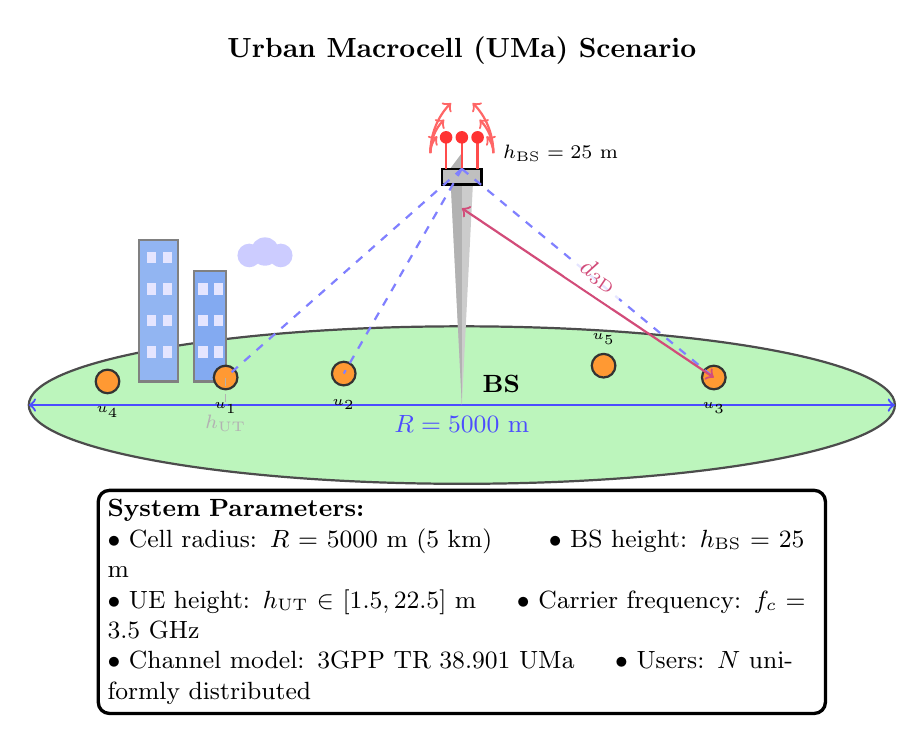
\begin{tikzpicture}[
    scale=1.0, every node/.style={scale=1.0}
]

% Define colors
\definecolor{skyblue}{RGB}{135,206,235}
\definecolor{groundgreen}{RGB}{144,238,144}
\definecolor{building}{RGB}{100,149,237}

% Ground circle (cell coverage)
\fill[groundgreen!60] (0,0) ellipse (5.5cm and 1cm);
\draw[thick, black!70] (0,0) ellipse (5.5cm and 1cm);

% Cell radius annotation
\draw[<->, thick, blue!70] (-5.5,-0) -- (5.5,-0) node[midway, below, font=\small] { $R = 5000$ m};

% Base Station Tower (CENTER)
\begin{scope}[xshift=0cm]
    % Tower structure
    \fill[gray!40] (0,0) -- (-0.15,3) -- (0.15,3) -- cycle;
    \fill[gray!60] (0,0) -- (-0.15,3) -- (0,3.2) -- cycle;
    
    % Platform at top
    \draw[fill=gray!50, thick] (-0.25,2.8) rectangle (0.25,3);
    
    % Antenna elements
    \foreach \x in {-0.2,0,0.2} {
        \draw[thick, red!70] (\x,3) -- (\x,3.4);
        \fill[red!80] (\x,3.4) circle (0.08);
    }
    
    % Signal waves
    \foreach \i in {1,2,3} {
        \draw[thick, red!60, ->] (-0.4,3.2) arc[start angle=180, end angle=135, radius=0.3*\i];
        \draw[thick, red!60, ->] (0.4,3.2) arc[start angle=0, end angle=45, radius=0.3*\i];
    }
    
    % BS label
    \node[font=\small\bfseries, below] at (0.5,0.5) {BS};
    \node[font=\scriptsize, right] at (0.4,3.2) {$h_{\mathrm{BS}} = 25$ m};
\end{scope}

% Buildings (left side)
\begin{scope}[xshift=-3.5cm, yshift=0.3cm]
    % Building 1
    \fill[building!70] (-0.6,0) rectangle (-0.1,1.8);
    \draw[thick, black!50] (-0.6,0) rectangle (-0.1,1.8);
    % Windows
    \foreach \y in {0.3,0.7,1.1,1.5} {
        \foreach \x in {-0.5,-0.3} {
            \fill[white!90!blue] (\x,\y) rectangle (\x+0.12,\y+0.15);
        }
    }
    
    % Building 2
    \fill[building!80] (0.1,0) rectangle (0.5,1.4);
    \draw[thick, black!50] (0.1,0) rectangle (0.5,1.4);
    % Windows
    \foreach \y in {0.3,0.7,1.1} {
        \foreach \x in {0.15,0.35} {
            \fill[white!90!blue] (\x,\y) rectangle (\x+0.12,\y+0.15);
        }
    }
    
    % Small cloud
    \fill[white!80!blue] (0.8,1.6) circle (0.15);
    \fill[white!80!blue] (1,1.65) circle (0.18);
    \fill[white!80!blue] (1.2,1.6) circle (0.15);
\end{scope}

% Users (UEs) distributed in cell
\begin{scope}
    % User 1 (near buildings, weak user)
    \fill[orange!80] (-3,0.35) circle (0.15);
    \draw[thick, black!80] (-3,0.35) circle (0.15);
    \node[font=\tiny, below] at (-3,0.15) {$u_1$};
    \draw[dashed, gray!60] (-3,0.35) -- (-3,0) node[below, font=\scriptsize] {$h_{\mathrm{UT}}$};
    
    % User 2 (middle-left)
    \fill[orange!80] (-1.5,0.4) circle (0.15);
    \draw[thick, black!80] (-1.5,0.4) circle (0.15);
    \node[font=\tiny, below] at (-1.5,0.2) {$u_2$};
    
    % User 3 (right, strong user) - for d3D annotation
    \fill[orange!80] (3.2,0.35) circle (0.15);
    \draw[thick, black!80] (3.2,0.35) circle (0.15);
    \node[font=\tiny, below] at (3.2,0.15) {$u_3$};
    
    % User 4 (far edge left)
    \fill[orange!80] (-4.5,0.3) circle (0.15);
    \draw[thick, black!80] (-4.5,0.3) circle (0.15);
    \node[font=\tiny, below] at (-4.5,0.1) {$u_4$};
    
    % User 5 (top right)
    \fill[orange!80] (1.8,0.5) circle (0.15);
    \draw[thick, black!80] (1.8,0.5) circle (0.15);
    \node[font=\tiny, above] at (1.8,0.65) {$u_5$};
\end{scope}

% Communication links (dashed lines from BS to users)
\draw[thick, dashed, blue!50] (0,3) -- (-3,0.35);
\draw[thick, dashed, blue!50] (0,3) -- (-1.5,0.4);
\draw[thick, dashed, blue!50] (0,3) -- (3.2,0.35);

% Distance annotations - d3D (3D distance from BS to user)
\draw[<->, thick, purple!70] (0,2.5) -- (3.2,0.35) node[midway, above, font=\small, sloped, fill=white, fill opacity=0.8, text opacity=1] {$d_{3\mathrm{D}}$};

% Title
\node[font=\normalsize\bfseries] at (0,4.5) {Urban Macrocell (UMa) Scenario};

% System parameters box
\node[draw, very thick, fill=white, rectangle, text width=90mm, font=\small, align=left, rounded corners] at (0,-2.5cm) {
\textbf{System Parameters:}\\
$\bullet$ Cell radius: $R = 5000$ m (5 km) \hspace{5mm} $\bullet$ BS height: $h_{\mathrm{BS}} = 25$ m\\
$\bullet$ UE height: $h_{\mathrm{UT}} \in [1.5, 22.5]$ m \hspace{3mm} $\bullet$ Carrier frequency: $f_c = 3.5$ GHz\\
$\bullet$ Channel model: 3GPP TR 38.901 UMa \hspace{3mm} $\bullet$ Users: $N$ uniformly distributed
};

\end{tikzpicture}
